\subsubsection{Πρόβλεψη με χρήση General-inflated Generalized Poisson μοντέλου} \label{section:GIGP}
Η στατιστική ανάλυση θετικών και ακεραίων τιμών, οι οποίες στη βιβλιογραφία περιγράφονται ως μεταβλητές πλήθους (count variables) γίνεται με χρήση κατανομών όπως η Poisson και η αρνητική διωνυμική. Καθώς οι κατανομές αυτές περιέχουν ένα μικρό πλήθος παραμέτρων έχει διαπιστωθεί πως δεν είναι επαρκείς για τη περιγραφή της διακύμανσης σε πραγματικά σετ δεδομένων. Τα Γενικευμένα μοντέλα \citep{Neld:Wedd:1972} εισήχθησαν προκειμένου να αντιμετωπιστεί αυτό το πρόβλημα με χρήση βαρών σε μεταβλητές προβλέπτες. Ενώ λοιπόν το μοντέλο Poisson περιγράφεται από τη συνάρτηση μάζας πιθανότητας:

\begin{equation}
 p(\kappa \mid \lambda) = \frac{\lambda^\kappa}{\kappa!} e^{-\lambda}
 \label{eq:poisson}
\end{equation}   

όπου $\kappa$ το ζητούμενο σημείο και $\lambda$ η μέση τιμή της κατανομής, το Γενικευμένο μοντέλο διατυπώνεται ως εξής:

\begin{equation}
 p(\kappa \mid \lambda, \alpha) = \frac{\mu_k}{1+\alpha \mu_k} ^k \frac{1+\alpha k}{k!}^{k-1} e^{\frac{-\mu_k(1+\alpha y_k)}{1+\alpha \mu_k}}
 \label{eq:gpoisson}
\end{equation}

όπου $\mu_k(x_k) = e^{\sum_{}^{} x_{ij} \beta_j}$, με $x_{ij}$ τις τιμές των μεταβλητών προβλεπτών και $\beta$ τα βάρη τους. Η παράμετρος $\alpha$ ρυθμίζει την υπερ-διακύμανση (overdispersion) του μοντέλου.

Η διαπίστωση παρουσίας εκτεταμένους πλήθους μηδενικών τιμών σε πολλά πραγματικά προβλήματα οδήγησε στο σχηματισμό των zero-inflated poisson μοντέλων \citep{Lambert:1992:ZPR:149268.149270}, που προσπαθούν να διορθώσουν την υπερ-διακύμανση υπολογίζοντας ένα μοντέλο για τα μηδενικά και ένα για τις υπόλοιπες τιμές. Ο \citet{gip} γενικεύει τα μοντέλα αυτά διατυπώνοντας τη συνάρτηση πυκνότητας πιθανότητας ενός general-inflated poisson μοντέλου, δηλαδή ενός μοντέλου το οποίο μπορεί να προσαυξηθεί με κατανομές σε οποιοδήποτε σημείο συσσώρευσης τιμών, ως εξής: 
\begin{equation}
 p(\kappa \mid \lambda, \pi_i, 1 \leq i \leq m) = \begin{cases}
 \pi_i + (1-\sum_{i=1}^{m} \pi_i) p(\kappa \mid \lambda) , & \text{εάν $k=k_1, \cdots, k_m$}.\\
 (1-\sum_{i=1}^{m} \pi_i) p(\kappa \mid \lambda), & \text{εάν $k \neq k_i, 1 \leq i \leq m$}.
 \end{cases}
\end{equation}

όπου $p(\kappa \mid \lambda)$ η Poisson συνάρτηση μάζας πιθανότητας όπως αυτή ορίζεται στην Εξίσωση \ref{eq:poisson} και $\pi_i$ μία παράμετρος που ορίζει τη μάζα στο σημείο συσσώρευσης $i$ από τα συνολικά $m$.

Οι \citet{Famoye_onthe} περιγράφουν τα zero-inflated Generalized Poisson μοντέλα, ένα συνδυασμό μεθόδων για την αντιμετώπιση της υπερ-διακύμανσης και του εκτεταμένου πλήθους μηδενικών. 

Για τις ανάγκες του προβλήματος που αντιμετωπίζουμε θα ορίσουμε το General-inflated Genera\-lized Poisson μοντέλο, προκειμένου να εκμεταλλευτούμε τα μετα-χαρακτηριστικά και να αντιμετωπίσουμε την συσσώρευση τιμών στο 4. Προς αυτό το σκοπό θα συνδυάσουμε τα δύο προηγούμενα μοντέλα στην ακόλουθη συνάρτηση μάζας πιθανότητας:

\begin{equation}
 p(\kappa \mid \lambda, \phi_i, 1 \leq i \leq m) = \begin{cases}
 \phi_i + (1-\sum_{i=1}^{m} \phi_i) p(\kappa \mid \lambda, \alpha) , & \text{εάν $k=k_1, \cdots, k_m$}.\\
 (1-\sum_{i=1}^{m} \phi_i) p(\kappa \mid \lambda, \alpha), & \text{εάν $k \neq k_i, 1 \leq i \leq m$}.
 \end{cases}
\end{equation} 
 
 όπου $p(\kappa \mid \lambda, \alpha)$ η Generalized Poisson συνάρτηση μάζας πιθανότητας όπως αυτή ορίζεται στην Εξίσωση \ref{eq:gpoisson} και $\pi_i$ μία παράμετρος που ορίζει τη μάζα στο σημείο συσσώρευσης $i$ από τα συνολικά $m$.
 
 Βασισμένοι στα πειράματα των \citep{gip} και \citep{Famoye_onthe} ακολουθήσαμε την ακόλουθη διαδικασία για την προσαρμογή ενός General-inflated Generalized Poisson μοντέλου στα δεδομένα μας:
 \begin{itemize}
 	\item Προσαρμογή ενός Generalized Poisson μοντέλου για την εύρεση αρχικών τιμών για $\alpha$, $\beta$.
 	\item Προσαρμογή ενός General-inflated Poisson μοντέλου για την εύρεση των αρχικών τιμών των $\pi$.
 	\item Χρήση των αρχικών τιμών για προσαρμογή ενός General-inflated Generalized Poisson μοντέλου.
 \end{itemize}
 
 Η προσαρμογή των μοντέλων γίνεται βελτιστοποιώντας τις παραμέτρους με χρήση της τεχνικής Maximum Likelihood Estimation με αλγόριθμο αναζήτησης τη μέθοδο Nelder-Mead. Καθώς ο αλγόριθμος αυτός είναι ευαίσθητος στις αρχικές τιμές των παραμέτρων πραγματοποιήσαμε cross-validation σε ένα πλέγμα αρχικών τιμών για τα βήματα 1 και 2. Στα διάγραμματα \ref{fig:low} και \ref{fig:high} βλέπουμε τη συνάρτηση μάζας πιθανότητας του προσαρμοσμένου μοντέλου και τις πραγματικές συχνότητες των δεδομένων μας:
 
\begin{figure}[!htb]
	\begin{minipage}{0.48\textwidth}
		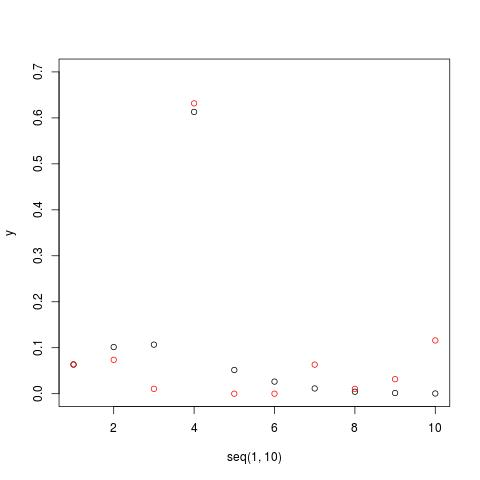
\includegraphics[width=0.9\textwidth]{gigp_low}
		\caption{Σύγκριση General-inflated Generalized Poisson συνάρτηση μάζας πιθανότητες με πραγματικές συχνότητες: Αρχικοποίηση που προσαρμόζεται καλά στο σημείο συσσώρευσης και στις χαμηλές τιμές.}	
		\label{fig:low}
	\end{minipage}
	\begin{minipage}{0.48\textwidth}
		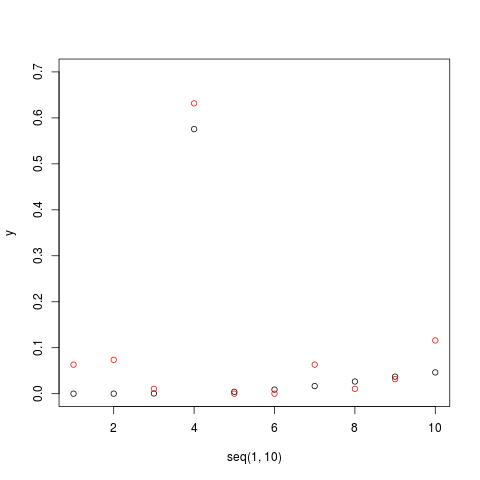
\includegraphics[width=0.9\textwidth]{gigp_high}
		\caption{Σύγκριση General-inflated Generalized Poisson συνάρτηση μάζας πιθανότητες με πραγματικές συχνότητες: Αρχικοποίηση που προσαρμόζεται καλά στο σημείο συσσώρευσης και στις υψηλές τιμές.}	
		\label{fig:high}
	\end{minipage}
\end{figure}
\FloatBarrier
